% Die Vorlage fuer Abschlussarbeiten benutzt die hervorragende
% Klasse ``hepthesis'' von Andy Buckley
% zusammengestellt von : Felix Richter, 02.03.2010

%\documentclass[12pt,twoside,bind,ams,a4paper,hyper]{hepthesis}
\documentclass[12pt,twoside,bind,ams,a4paper]{hepthesis}

% Unicode(UTF-8)-Kodierung anschalten. Damit koennen dann alle
% deutschen Umlaute und fremdsprachlichen Zeichen direkt verwendet werden (z.B. - statt \"A)
% es muss allerdings ein unicode-faehiger Editor benutzt werden (unter Linux alle, unter Windows ???).
\usepackage[utf8]{inputenc}
\usepackage[T1]{fontenc}

% fuer eine Arbeit in deutscher Sprache sinnvoll:
\usepackage[ngerman]{babel}

% Schriftarten: Variante 1
\usepackage{lmodern,hfoldsty,charter}
% Schriftarten: Variante 2
%\usepackage{charter}

% Paket fuer mathematische Symbole
\usepackage{amssymb}

% Paket fuer Literaturverzeichnis nach DIN
\usepackage{natbib}
% Literaturzitate in eckige Klammern setzen
\setcitestyle{square}

% Paket zum Einbinden von ein- oder mehrseitigen PDFs
\usepackage{pdfpages}

\usepackage{url}

% Paket zur typographisch richtigen Angabe von Groessen mit SI-Masseinheiten
\usepackage[squaren]{SIunits}

% Paket fuer Bra-/Ket-Vektor-Schreibweise, mit automatischer Groessenanpassung
\usepackage{braket}

\title{Thema der Arbeit}
\author{Kirstin Schulz}

% Die folgenden Zeilen aktivieren, wenn ein PDF mit anklickbarem Inhaltsverzeichnis
% sowie anklickbaren Verweisen auf Gleichungen und Literaturhinweise erzeugt werden soll.
% Die folgenden Zeilen auskommentieren, wenn ein PDF zum reinen Ausdruck erzeugt werden soll.
% Zusaetzlich muss oben im documentclass-Befehl, die Option ``hyper'' herausgenommen  
% bzw. hinzugefuegt werden.
%\hypersetup{
% pdfauthor = {\theauthor},
% pdftitle = {\thetitle},
% pdfsubject = {Master's thesis, University of Rostock, Germany, 2010},
% bookmarksopen=true
%}


% Zeilenanstaende -- eins der folgenden auswaehlen. 1 1/2 ist Voreinstellung, sollte 
% beibehalten werden.

%\setmainmatterspacing{single}
%\setmainmatterspacing{onehalf}
%\setmainmatterspacing{double}

\begin{document}

\begin{frontmatter}
% ``klassisches'', vollstaendig in Latex gesetztes Titelblatt
% Klassische Titelseite

\thispagestyle{empty}
\begin{center}
\vspace*{-2cm}

\includegraphics[width=0.75\textwidth]{unilogo-siegel-farbe}\\
\vspace*{3cm}
    {\titlefont \huge \onehalfspacing
	\thetitle 
    \par}%
   \vfill
%  \vskip 6em
    {\normalfont\normalcolor\bfseries
	\large
	Dissertation \\
	\large
%	im Studiengang Physik\\
	zur\\
	Erlangung des akademischen Grades\\
	doctor rerum naturalium (Dr. rer. nat.)\\ 
	der Mathematisch-Naturwissenschaftlichen Fakultät\\
	der Universität Rostock
    \par}%
\end{center}\par
%\vfill
\vspace*{2.5cm}
\noindent\begin{minipage}[b]{\textwidth}
{\bf
  \noindent vorgelegt von\\
  Kirstin Schulz, geb.~am 10.~Januar 1988 in 
Clausthal-Zellerfeld\\

%%% Nur für Pflichexemplare

%  \begin{tabbing}
%  Betreuer und 1.~Pr\"ufer :  \= PD Dr. Lars Umlauf, Leibniz Institut für 
%Ostseeforschung\\
% 2.~Pr\"ufer: \> ???, Universität Rostock \\
%  \end{tabbing}

  \noindent Rostock, den 07. Oktober 2016
  }
\end{minipage}




% Alternative: Titelblatt im Uni-Corporate-Design aus Word/OpenOffice-Vorlage erstellen,
% als PDF abspeichern/exportieren und hier mit pdfpages einbinden.
% \includepdf[pages={1}]{titelseite-cd.pdf}


\begin{abstract}[Abstract]
\thispagestyle{plain}
Sediment transport is governed by the complex interplay of many different 
processes. Near sloping topography, sediment transport can be triggered by 
asymmetries in the density stratification during an oscillatory current going 
up and down the slope. This process was investigated in detail by means of an 
idealized numerical model. It was found that the process depends on the 
strength of the vertical stratification and the slope angle, and residual 
sediment transport is directed upslope for most of the parameter constellations. 
A more profound numerical model was used to successfully reproduce observations 
of this process from the East China Sea, and to investigate the effect of Earth 
rotation. Another data set was analyzed to investigate sediment dynamics 
across the rim of a deep basin in the Baltic Sea. It was found that parts of 
the sediment transported there are dispersed across the bottom slope into 
shallower areas.
\end{abstract}


\begin{abstract}[Zusammenfassung]
\thispagestyle{plain}
\sloppy
Der Transport von Sedimenten wird von dem komplexen Zusammenspiel vieler 
verschiedener Prozesse bestimmt. Nahe eines geneigten Meeresbodens können 
Asymmetrien in der vertikalen Dichteschichtung während der Phasen einer 
oszillierenden Strömung quer zum Hang einen residuellen Sedimenttransport 
verursachen. Dieser Prozess wurde mit der Hilfe eines idealisierten numerischen 
Modells detailliert untersucht. Es hat sich gezeigt, dass die Stärke der 
vertikalen Dichteschichtung und der Winkel des Hanges großen Einfluss auf 
diesen Prozess haben, der residuelle Sedimenttransport aber für den Großteil 
der Parameterkombinationen hangaufwärts gerichtet ist. Das Modell wurde 
erweitert, um erfolgreich Beobachtungen dieses Prozesses aus dem 
Ostchinesischen Meer zu reproduzieren und um den Einfluss der Erdrotation zu 
bestimmen. Ein weiteres Datenset wurde analysiert um die Sedimentdynamik 
am Hang eines tiefen Beckens in der Ostsee zu untersuchen. Es wurde 
herausgefunden, das Sediment, welches einmal in das Becken hinein transportiert 
wurde, auch wieder in Richtung flacherer Gebiete verteilt werden kann.
\fussy
\end{abstract}

\cleardoublepage

\thispagestyle{plain}

\begin{center}
 \textbf{Acknowledgements}
\end{center}

I like to express my deep gratitude to the people who surrounded and supported 
me during my PhD time. In the last three years I did not only get to know a 
totally new field of scientific work, but I met unbelievably wonderful 
people that made my time in Rostock to be a great experience. 

In first place, I thank my supervisor Lars Umlauf, who invested so much time 
and energy to make a physicist out of me. Thank you for encouraging me all the 
time and thank you for all your advice, and for helping me through the hard 
times when nothing went right.

I also thank the other three members of my thesis committee: Hans Burchard, 
thank you for introducing me to all the people on the conferences and for 
always offering your help. You were like a second supervisor for me. Henk 
Schuttelaars, thank you for all the wonderful conversations, in Havard as well 
as on the Christmas Market, and your advice on my work and my future. And 
finally Gregor Rehder, who was the most sympathetic chief scientist I ever went 
on a cruise with. 

I greatly thank my working group and the colleagues from the project. Thanks 
to all the people that shared some time in room 214 with me: Mahdi 
Mohammadi-Aragh, who helped me so much during my first time and provided me with 
the most important schedule ever, Kaveh Purkiani and Johannes Becherer, Merten 
Siegfried, Selina Müller and Madline Kniebusch, who all contributed to the 
familiar and relaxed atmosphere in our office. Special thanks goes to Chris 
Lappe, who untiringly answered all my questions about oceanography and who tried 
to explain internal waves to me at least a hundred times. Thanks to GETMan Knut 
Klingbeil, for permanent support with everything related to computers, and for 
your ability to encourage me. Thanks to Elisabeth Schulz, who I always looked up 
to. Thanks to Peter Holtermann for showing me Galvano, to Ulf Gräwe, 
Xaver Lange and Berkay Basdurak for providing support and a wonderful and 
relaxed working atmosphere. Thanks to Berit Recklebe for being the shield to 
protect me from administration and for being a friend from my first working day 
on. I also want to thank Toralf Heene and Sebastian Beier for the technical 
support and their patience with me, and of course the crew members of the 
research vessels Alkor, Elisabeth Mann Borgese and Maria S. Merian. Thanks to 
my biologist Dr. David Kaiser, and Claudia Morys, Dennis Bunke, Jana Wölfel, 
Mayya Gogina, Florian Cordes and Julia Regnery, who made the ships cruises an 
unforgettable experience and became my closest friends during my time in 
Rostock.\newpage
\thispagestyle{plain} I am so grateful that I had the opportunity to meet all of 
you and I hope we will stay in touch.

I also want to express my gratitude to Prof. Dr. Margit Rösler, who was my 
mentor during my years at the Technical University of Clausthal-Zellerfeld, and 
who taught me to never surrender to a problem. I would also like to thank 
Wiebke Klünder and Markus Schreiber for always being there for me, during study 
times and beyond.

In the end, I want to thank my perfect flatmate Josephina Seltenheim, for 
providing me shelter when I came to Rostock and for being such a wonderful 
person, and all my other friends in Berlin. I always loved to have you around. 
I want to thank my best friend Jennifer Smoch for your endless support with 
anything and the wonderful times we have together and my partner Christian 
Meier for his patience and for moving to the Netherlands with me. I thank my 
family, my grandmother Eva Eggeling and especially my mother Maike, 
for creating a wonderful childhood for me and for supporting me in every 
possible way. Everything I have achieved so far I owe to you. I thank my amazing 
brother Paul for all the years we have been together and my father Uwe for 
everything he did for me. Finally, I particularly want to thank Marko 
Lipka, who shared his apartment, Socke the dog and his small family with me for 
the last two years. You and Klara were such a huge and wonderful part of my 
life here and I will miss you so much. Goodbye und Guten Flug. 

\textbf{Regarding the publications in chapter 2 and 3:} These studies were 
carried out in the context of the interdisciplinary project SECOS, funded by the 
German Federal Ministry of Education and Research under grant 03F0666A, WP 2.1 
(PI: Lars Umlauf). We are grateful to Henk Schuttelaars (TU Delft), Hans
Burchard, Ulf Gr{\"a}we, Knut Klingbeil, and Jan-Torben Witte (all IOW) for 
modeling support and helpful comments on the manuscripts.  Computations were
carried out with a modified version of General Ocean Turbulence Model
(GOTM, www.gotm.net) with the SPM component implemented using the
Framework for Aquatic Biogeochemical Models (FABM,
www.sf.net/projects/fabm). Observational data used in chapter \ref{kap-jgr} are
available from co-author T.\ Endoh upon request

\newpage

\tableofcontents

\end{frontmatter}

\begin{mainmatter}
\chapter{The Baltic Sea}
\label{kap-einleitung}

In the previous chapters, an idealized process study with the help of a 
numerical model was carried out (section \ref{kap-slope}) and observations of 
the discussed process in an existing data set from the East China Sea were 
reproduced (section \ref{kap-jgr}). Besides model studies, several field work 
campaigns were performed in the context of this thesis. The measurements were 
carried out in coastal areas of the Western Baltic Sea. Prior to the discussion 
of the obtained data in the next chapter, an introduction on the evolution of 
the Baltic Sea and the present hydrological conditions is given in this 
chapter, and the sedimentology and prevailing hydrodynamic processes which are 
characteristic in parts of the Western Baltic Sea are highlighted.

\section{History and Present State}

The Baltic Sea emerged from a subglacial lake at the end of the Weichselian Ice 
Age, approximately 12,000 BP, and has since gone through several stages of 
salty and brackish sea states or fresh water conditions, depending on whether a 
connection to the open ocean was established or not. Indicators for this 
alternations are, amongst others, changes in the benthic communities, and so the 
nomenclature of the evolution stages was often determined by the prevailing 
species.

With the retreat of the glaciers at the end of the Weichselian Ice Age, a 
subglacial lake, together with water from the rapidly melting glaciers, formed 
the \textit{Baltic Ice Lake}. Land uplift, that followed the deglaciation, 
formed a landbridge between Sweden and the main land 11,200 BP, damming the 
Baltic Ice Lake. Sea level was raised by glacial melt water until the lake began 
to drain over the Öresund sill. Presumably, a lowering of the water level by 25 
to 28 m by drainage through a channel near Mt. Billingen in central Sweden 
happened very rapidly around 10,300 BP, when the retreating ice margin collapsed 
\citep[][]{bjoerk95,tikkanen2002} and a connection to the sea was opened. 

This new stage of the Baltic with a lower sea level is known as \textit{Yoldia 
Sea} (from the marine mollusc \textit{Portlandia (Yolida) arctica} 
\citep[][]{schoning2001}). There are no indicators for salt water entrainment 
into the Yoldia Sea until global sea level rise and deglaciation formed a 
connection through the Närke Strait 300 years later \citep[][]{schoning2001}. 
This lead to brackish water conditions followed by decreasing salinity after the 
straits had become too narrow to allow water exchange another 100 to 300 years 
later \citep[][]{bjoerk95}.

After the glaciers retreated, uplift of the land was not be compensated by 
global sea level rise. Connection to the ocean was closed again around 9,500 BP, 
and the regime shifted to fresh water conditions again, now called 
\textit{Ancylus Lake} (after the freshwater gastropod \textit{Ancylus 
fluviatilis} \citep[][]{tikkanen2002}). Although narrow outlets existed, the 
surface of the Ancylus Lake rose up to 10 m above global sea level, inundating 
extensive areas of land. This phase, called the Ancylus Transgression, ended 
around 9,200 BP, when the sea level height exceeded the height of the Darss Sill 
and water began to flow out through an evolving river system in the land 
connection between Sweden and Germany \citep[][]{tikkanen2002}. Around 9,000 BP 
this so-called Ancylus Regression ended when the water level reached global sea 
level. The connection to the ocean through the river system remained, but no 
extensive saline intrusion happened for the next 1,000 years.

Ongoing global sea level rise deepened the connection between the Baltic Basin 
and the open ocean, letting more and more saline water enter the Ancylus Lake. A 
short transition stage called \textit{Mastogloia Sea} (\textit{Mastogloia} are 
diatoms that live in slightly saline conditions \citep[][]{eronen2001}) was 
followed by the \textit{Litorina Sea} (named after the brackish water gastropod 
\textit{Littorina littorea} \citep[][]{eronen2001}), when a great extent of 
saline water entered the Baltic basin through the Straits of Denmark in 7,500 BP 
\citep[][]{bjoerk95}. Transgression took place until the rise in ocean levels 
ended 6,000 to 5,000 BP. When the Straits of Denmark became shallower, as land 
uplift continued, water exchange was reduced and salinity in the Litorina Sea 
declined down to the present brackish state in 4,000 BP, at first named 
\textit{Limnea Sea} (from the snail \textit{Lymnaea ovata}), and finally, since 
500 BP, \textit{Mya Sea} (after the Northern American clam \textit{Mya 
arenaria}, which was brought into the Baltic by Viking ships 
\citep[][]{bjoerck2008}).

\begin{figure}[ht]
 \flushleft
 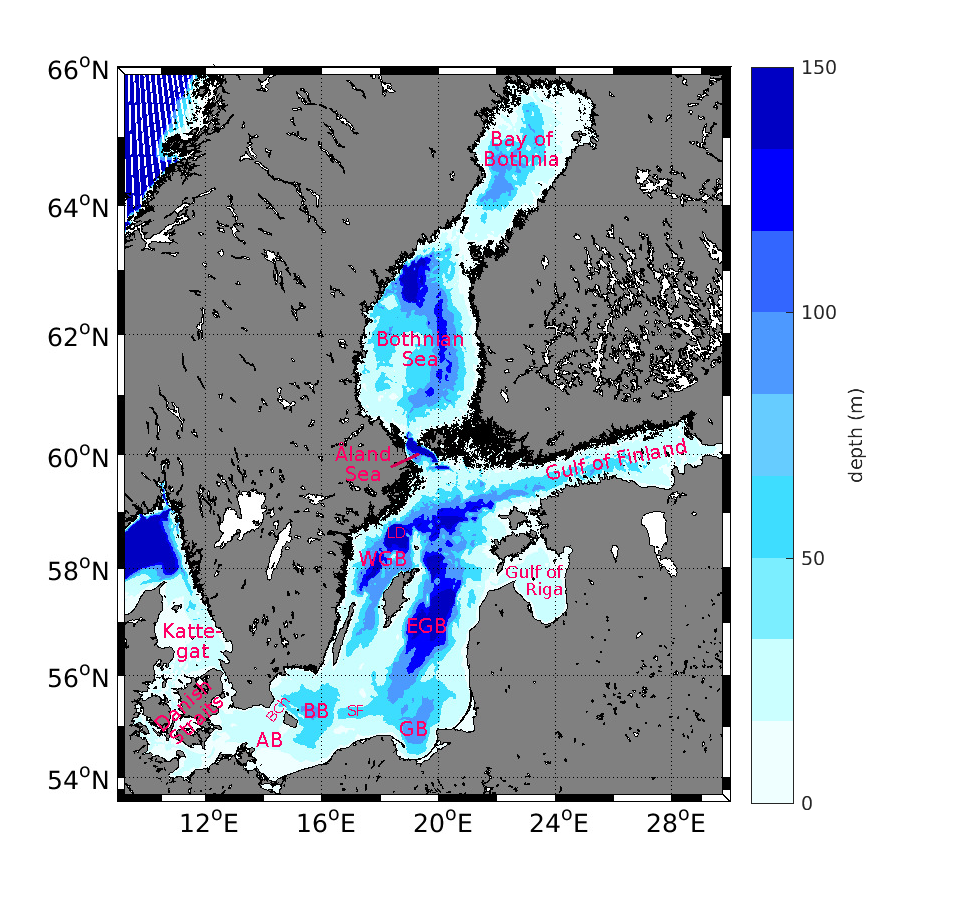
\includegraphics[width=17cm]{bilder/baltic.pdf}
 \caption{Topographic map of the Baltic Sea. Abbreviations stand for Arkona 
Basin (AB), Bornholm Channel (BCh), Bornholm Basin (BB), S\l upsk Furrow (SF), 
Gda\`{n}sk Basin (GB), Eastern Gotland Basin (EGB), Landsort Deep (LD) and 
Western Gotland Basin (WGB).}\label{balticmap}
\end{figure}

Today, the Baltic Sea has an extent of $4.2 \times 10^{5} \, \text{km}^2$ 
\citep[][]{balticsea} and is connected to the North Sea via the Danish Straits: 
the \O resund and the Great and Little Belt together with the Fehmarn Belt. The 
climate is humid: Annual precipitation adds around 224 $\text{km}^3$ of water to 
the Baltic Sea, evaporation amounts to only 184 $\text{km}^3$. River discharge a 
total of 436 $\text{km}^3$ water per year. \citep[][]{reissmann2009}. An 
exchange flow takes place, where brackish water leaves the Baltic near the 
surface (annually around 947 $\text{km}^3$) and saline North Sea water enters at 
the bottom (nearly 500 $\text{km}^3$ a year on average, but frequency and 
strength of inflow events differ dramatically over time, highly dependent on 
short term weather conditions). Two shallow sills, the Dr\o gden Sill (7 m deep, 
values in brackets refer to the local depth in the following) and the Darss Sill 
(18 m) form the passage to the first of several basins, the Arkona Basin (45 m), 
through which the North Sea water propagates as a deep gravity current 
(see \fig{balticmap}). Through 
the Bornholm Channel, the Arkona Basin is connected to the Bornholm Basin (80 
m), from where the bottom current flows over the S\l upsk Sill (60 m) and 
through the approximately 80 km long S\l upsk Furrow (90 m) southeast into the 
Gda\`{n}sk Basin (110 m) and northeast into the Eastern Gotland Basin (250 m). 
From there, the deep current can enter the easterly Gulf of Riga or the Western 
Gotland Basin, wherein the Landsort Deep (with 490 m the deepest point in the 
Baltic Sea) is located. The Gulf of Finnland forms the eastern boundary of the 
Baltic Sea and north of the Gotland Basin, the \r{A}land Sea separates the 
Baltic Proper in the south from the Bothnian Sea and the Bay of Bothnia in the 
north \citep[][]{reissmann2009}. Salt water entering at the Darss Sill needs 
approximately 2--6 months to exchange the bottom water in the Gotland Basin 
\citep[][]{balticsea}.

The bathymetry of the Baltic Basin together with climate conditions and the 
exclusive water exchange via the Danish Straits leads to several notable 
features in the hydrographic conditions: Dense bottom water from the North Sea 
creates a permanent strong halocline that separates bottom from surface water, 
preventing ventilation of the water masses in the deep basins. Oxygen that 
enters through exchange with the atmosphere is not mixed below the halocline, 
leaving entraining North Sea water the only oxygen source. Large parts of the 
Baltic Sea become anoxic after long periods without significant salt water 
inflows, with severe implications on geochemical processes and the ecosystem of 
both the lower water column and the sediment-water interface. 

Since the only source of saline water are inflows from the North Sea, a 
salinity gradient is present across the Baltic Sea: The bottom current is 
entrained with overlying brackish water along its pathway (for example, volume 
of the gravity current increases by 53 \% when passing through the Arkona Basin, 
\citep[see][]{reissmann2009}), and slow entrainment of salt into the overlying 
water mass forms a NE--SW surface salinity gradient. Surface salinity drops from 
around 18 psu in the Danish Straits to 8 psu in the Arkona Basin, down to 6--7 
psu in the Eastern Gotland Basin and even below 3 psu in the Bay of Bothnia and 
the Gulf of Finnland \citep[][]{balticsea}.

WAVE CLIMATE AND INERTIAL OSCILLATIONS GENERATION!

\section{Major Baltic Inflow December 2014}

GANZES KAPITEL WEG?

Saline water can enter the Baltic Sea in two different ways. Baroclinic inflows 
are triggered by the horizontal salinity gradient between North and Baltic Sea 
and occur at calm wind conditions, mostly in summer \citep[][]{reissmann2009}. 
The main impact on the ventilation of the deep sea is, however, subject to the 
barotropic inflow events, called Major Baltic Inflows (MBIs). Those MBIs occur 
irregularly and are caused by special meteorological conditions: Firstly, high 
air pressure over the Baltic region and strong winds in westerly direction cause 
the mean sea level in the Baltic to drop by up to 50 cm, imposing a gradient in 
sea level elevation between Kattegat and Arkona Basin. Secondly, several weeks 
of wind in easterly direction with strong gales \citep[][]{balticsea, 
reissmann2009, mohrholz2015} push saline and oxygen rich water into the Baltic 
Sea.
These conditions occur primarily between October and February. Since records 
started in 1897, MBIs were on a rather regular base up to the 1970s. After this, 
long periods without inflow events decreased oxygen supply in the Baltic basins 
drastically. The last MBIs were in 1993 and 2003, but they interrupted the 
anoxic conditions in the deep water only for short periods of time 
\citep[][]{schinke1998, mohrholz2015}.

In November 2014, medium to strong easterly winds forced an outflow of Baltic 
sea water and consequently a drop in mean sea level of 57 cm. At the beginning 
of December, the wind changed to heavily westerly wind, pushing a strong 
barotropic inflow of saline water into the Baltic Sea. The main inflow period 
lasted until Christmas. During that time, an overall amount of 320 $\text{km}^3$ 
water was imported into the Baltic Sea, carrying approximately 4 Gt salt. The 
MBI in 2014 was the third largest inflow event recorded since 1880 and has the 
potential to ventilate the entire deep water of the Baltic. 

\section{German Coastal Seas and Sediment}

General sedimentology and grain size distribution of parts of the Western 
Baltic Sea have 
been mapped in detail in a collaboration between the German maritime and 
hydrographic agency (BSH) and the Leibniz Institute for Baltic Sea Research 
(\fig{westernbaltic}). Prevailing sediments in this area reach from 
fine sand to silt. Although sediment distribution is rather inhomogeneous, some 
features related to the bathymetry are clearly visible. In the very shallow 
regions with water depth less than 20 m, predominately sandy sediments are 
found, while in the deeper basins finer silt is present.
As fine grained material is easily eroded, it is not likely to remain in highly 
energetic, shallow regions and is therefore transported into the deeper basins, 
where 
it accumulates \citep[][]{basys1}. This process is best visible at the 
transition from the Oder Bight to the Arkona Basin. It was found that the 20 m 
isobath separates erosional from depositional areas, and the muddy sediments 
accumulate below a regional halocline here \citep[][]{basys2}. MORE ON THE 
TW and AB REGION. TAUC ETC

\begin{figure}[ht]
 \flushleft
 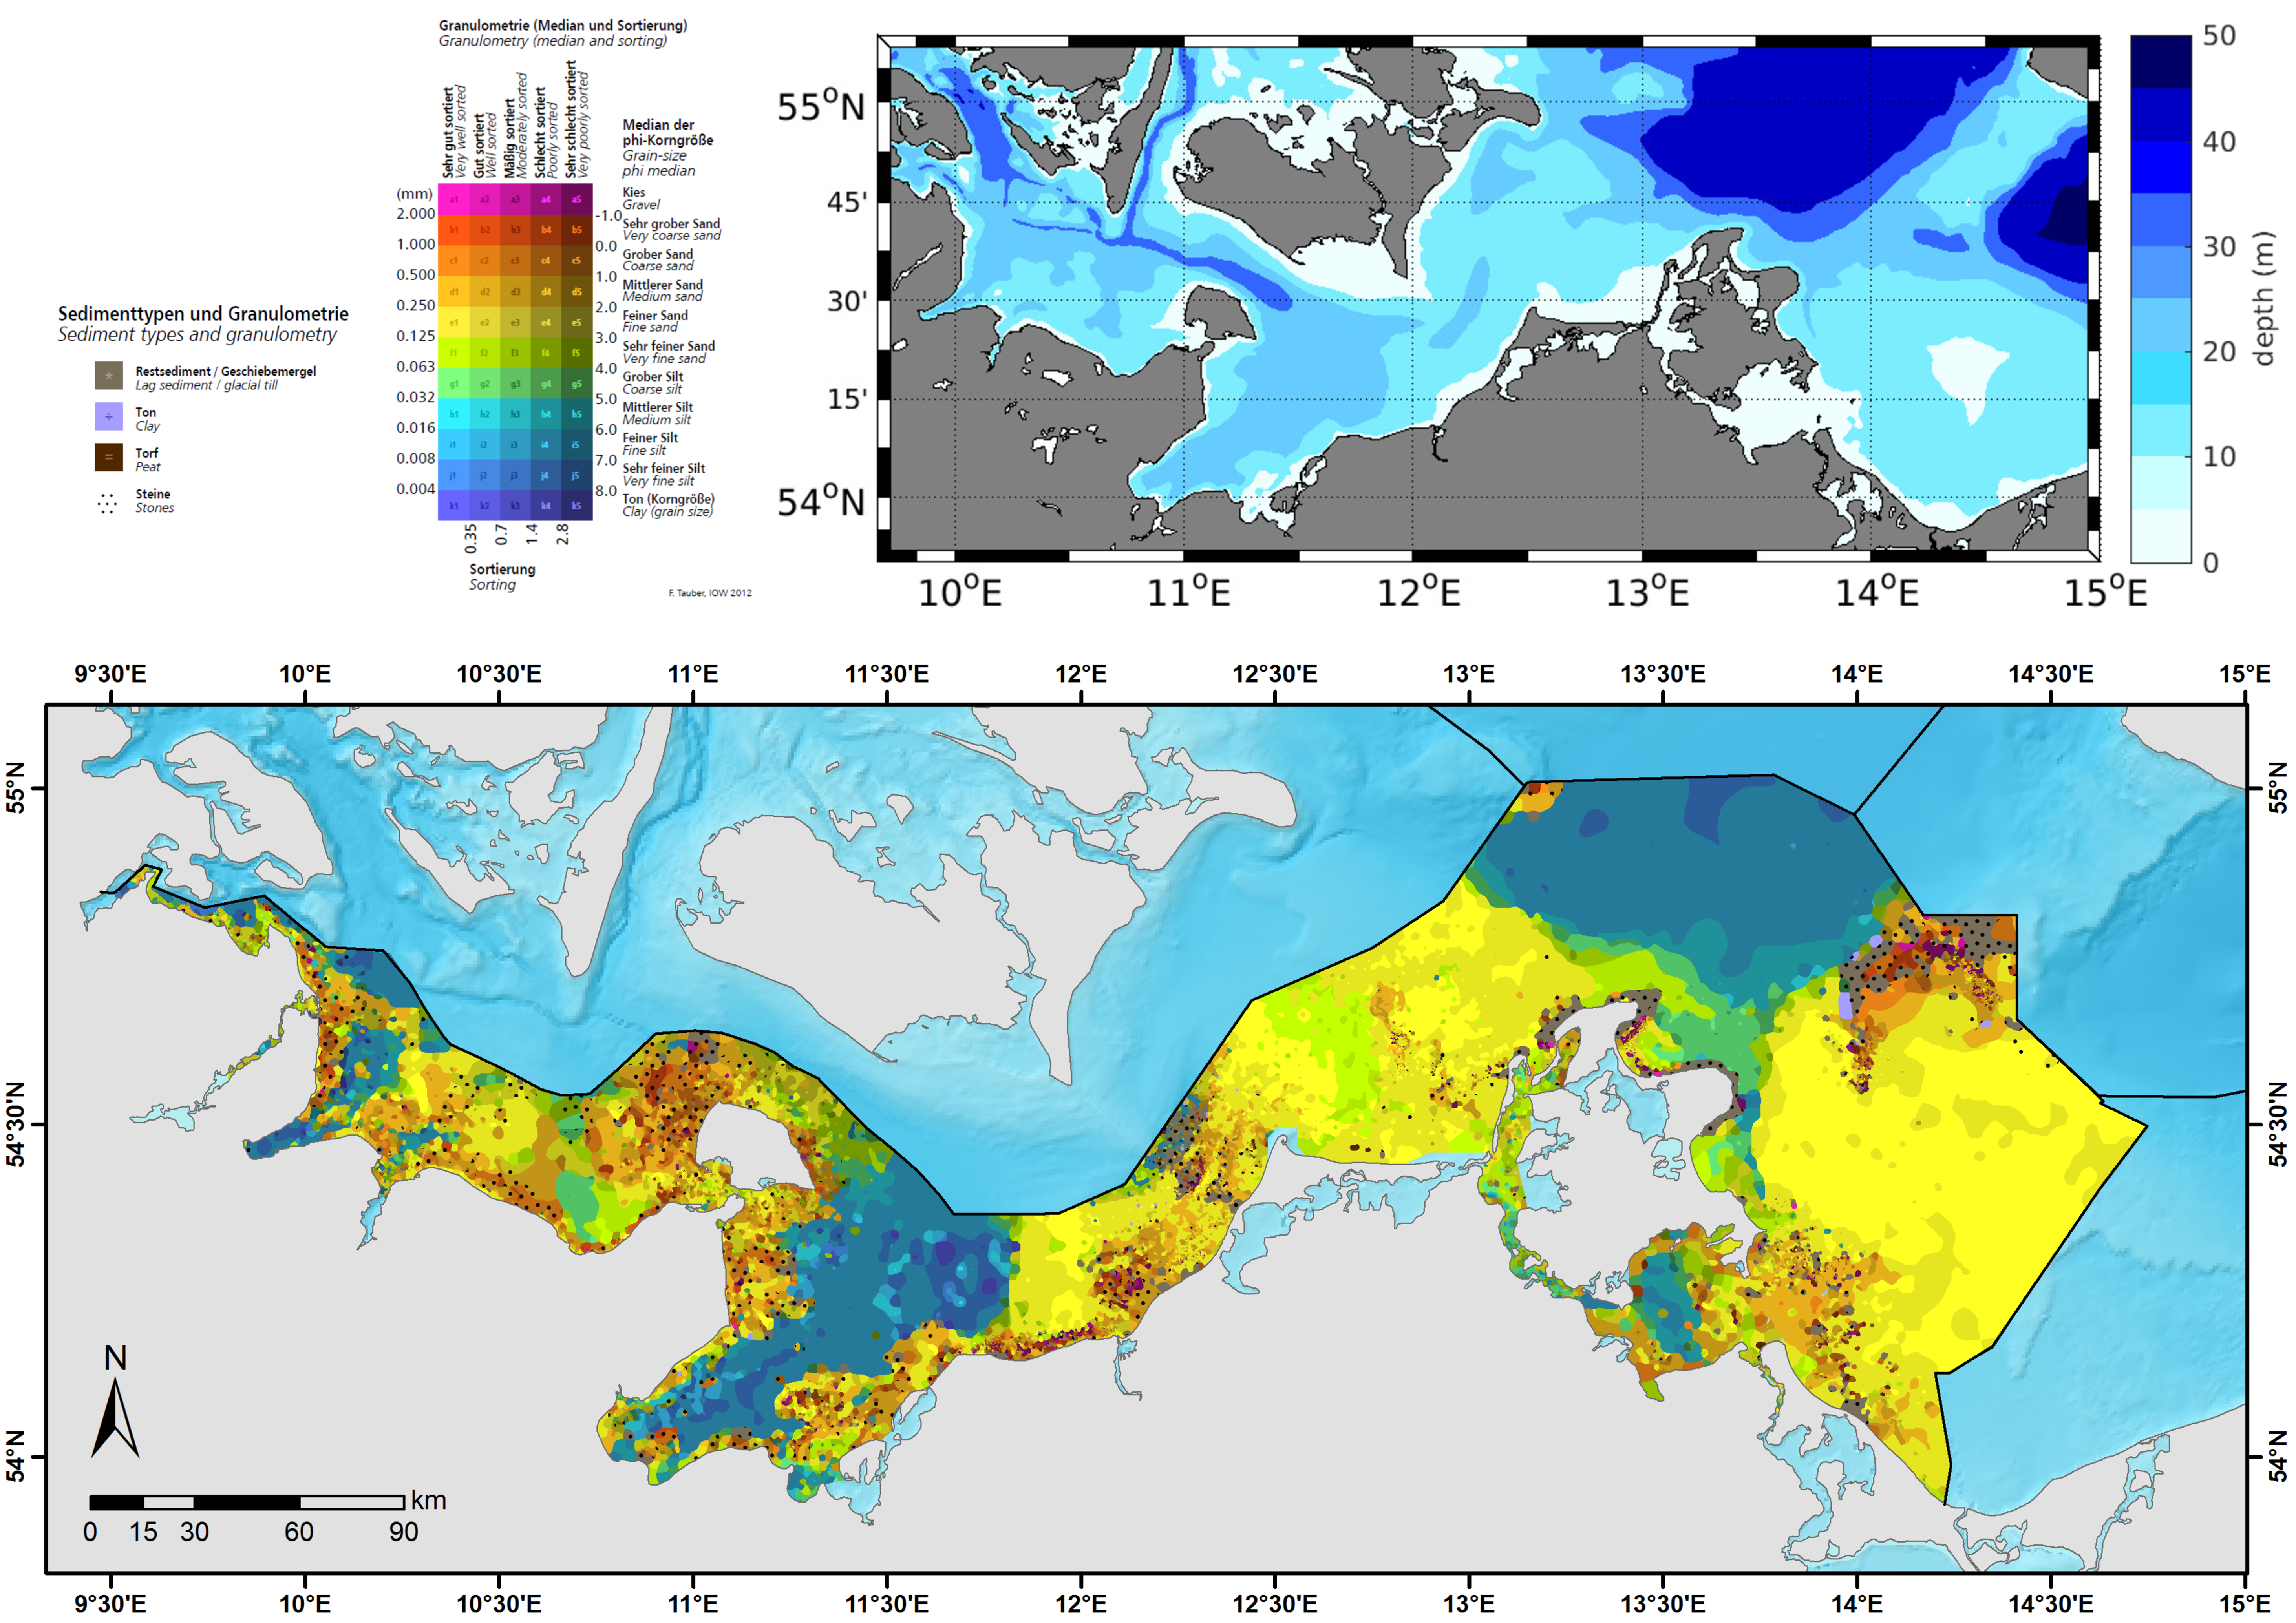
\includegraphics[width=15cm]{bilder/sediment.pdf}
 \caption{Topographic and sediment map of the Western Baltic 
Sea. Sediment data taken from \citep[][]{tauber2012}}\label{westernbaltic}
\end{figure}
\chapter{Measurements}
\label{kap-measure}

\section{Introduction}

\section{Study Area and Instrumentation}

We obtained hydrographic and turbulence data at 
several locations throughout the German coastal area during three cruises with 
R/V \textit{Alkor} in spring 2014 (AL434, 28.03.-08.04.2014), R/V 
\textit{Elisabeth Mann Borgese} in spring 2015 (EMB100, 09.04.-16.04.2015) and 
R/V \textit{Maria S. Merian} in winter 2016 (MSM50, 05.01.-29.01.2016). Here, 
we exclusively discuss data obtained in the transition zone from the coast off 
the island R\"{u}gen (called Tromper Wiek (TW), around 30~m water depth) to 
the approximately 45~m deep Arkona Basin (AB). The exact positions of deployed 
moorings and ship-based microstructure profiler transects are indicated in 
\fig{studyarea}.
 \begin{figure}[ht]
 \centering
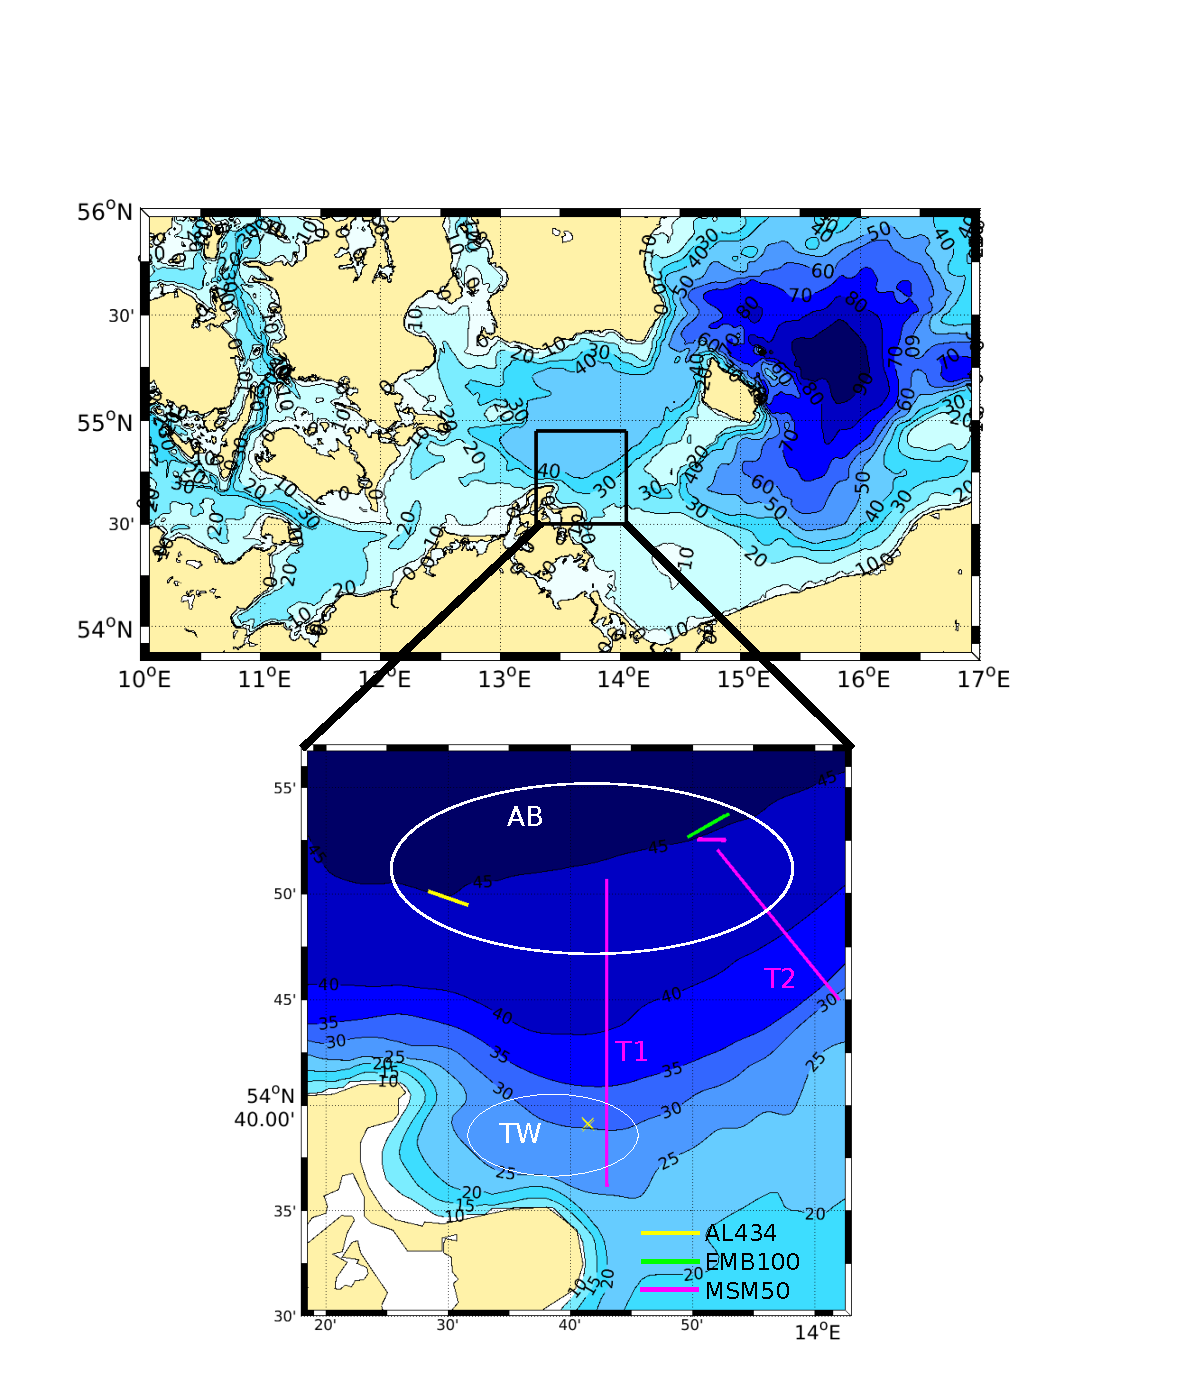
\includegraphics[width=17cm]{bilder/studyarea.pdf}
 \caption{Bathymetric map of the Western Baltic Sea and an enlargement of the 
study area. Deployments during cruise AL434 are indicated in yellow, from EMB100 
in green and from cruise MSM50 in magenta.}
 \label{studyarea}
 \end{figure}
 
 \begin{figure}[ht]
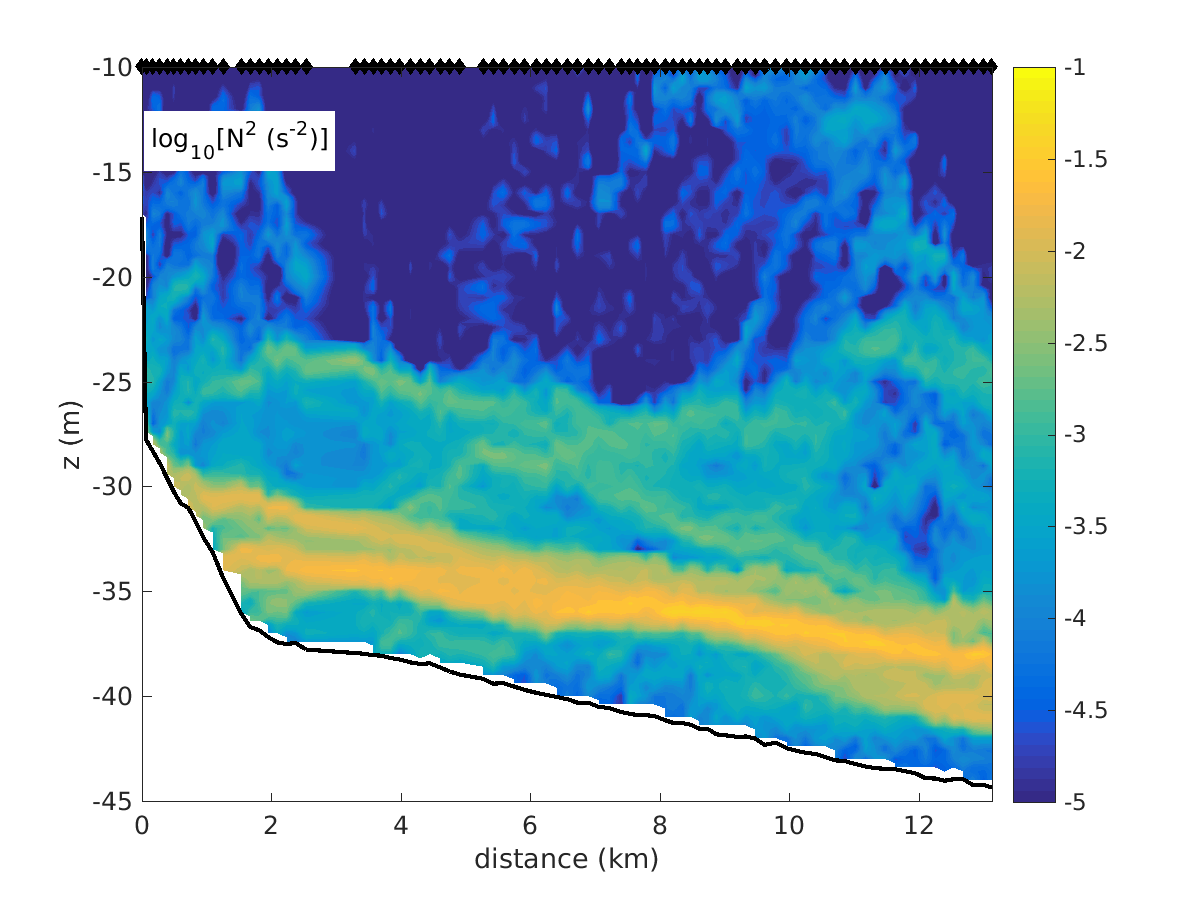
\includegraphics[width=40pc]{bilder/abslope.png}
 \caption{Topographic and hydrologic structure in the study area obtained from 
microstructure transect T1 in 2016. The steep slope on the left hand side has 
an inclination of approximately $5 \times 10^{-3}$, the mild slope further to 
the right of around $7 \times 10^{-4}$. Color indicates the buoynacy frequency 
$N^2$.}
 \label{abslope}
 \end{figure}

 Sediment distribution in this area is heterogeneous in the shallow regions 
with predominately medium to fine sand. At water depths below 25 - 30~m in the 
Arkona Basin, sediment is finer and consists homogeneously of silt 
(\fig{tauberkarte}). In the vicinity of TW, a special type of fine grained and 
organic poor sediment is found. Previous studies \citep[][]{leipe2000, 
basys1} found the Arkona Basin to be a deposition center for material 
orginiating from the shallower areas, with accumulation rates of around 2.2 
mm/yr. Sediment characteristics in the Arkona Basin resemble to those of a 
fluffy layer, i.e. it is easily resuspended and, due to its low settling 
velocity, remains suspended for a relatively long period of time. A consecutive 
study \citep[][]{basys2} found the 20~m isobath to be the border between 
erosional and depositional sites in this area, yielding that the Tromper Wiek 
region is depositional as well. This study also pointed out that muddy 
sediments accumulated below the halocline in this region.
 \begin{figure}[ht]
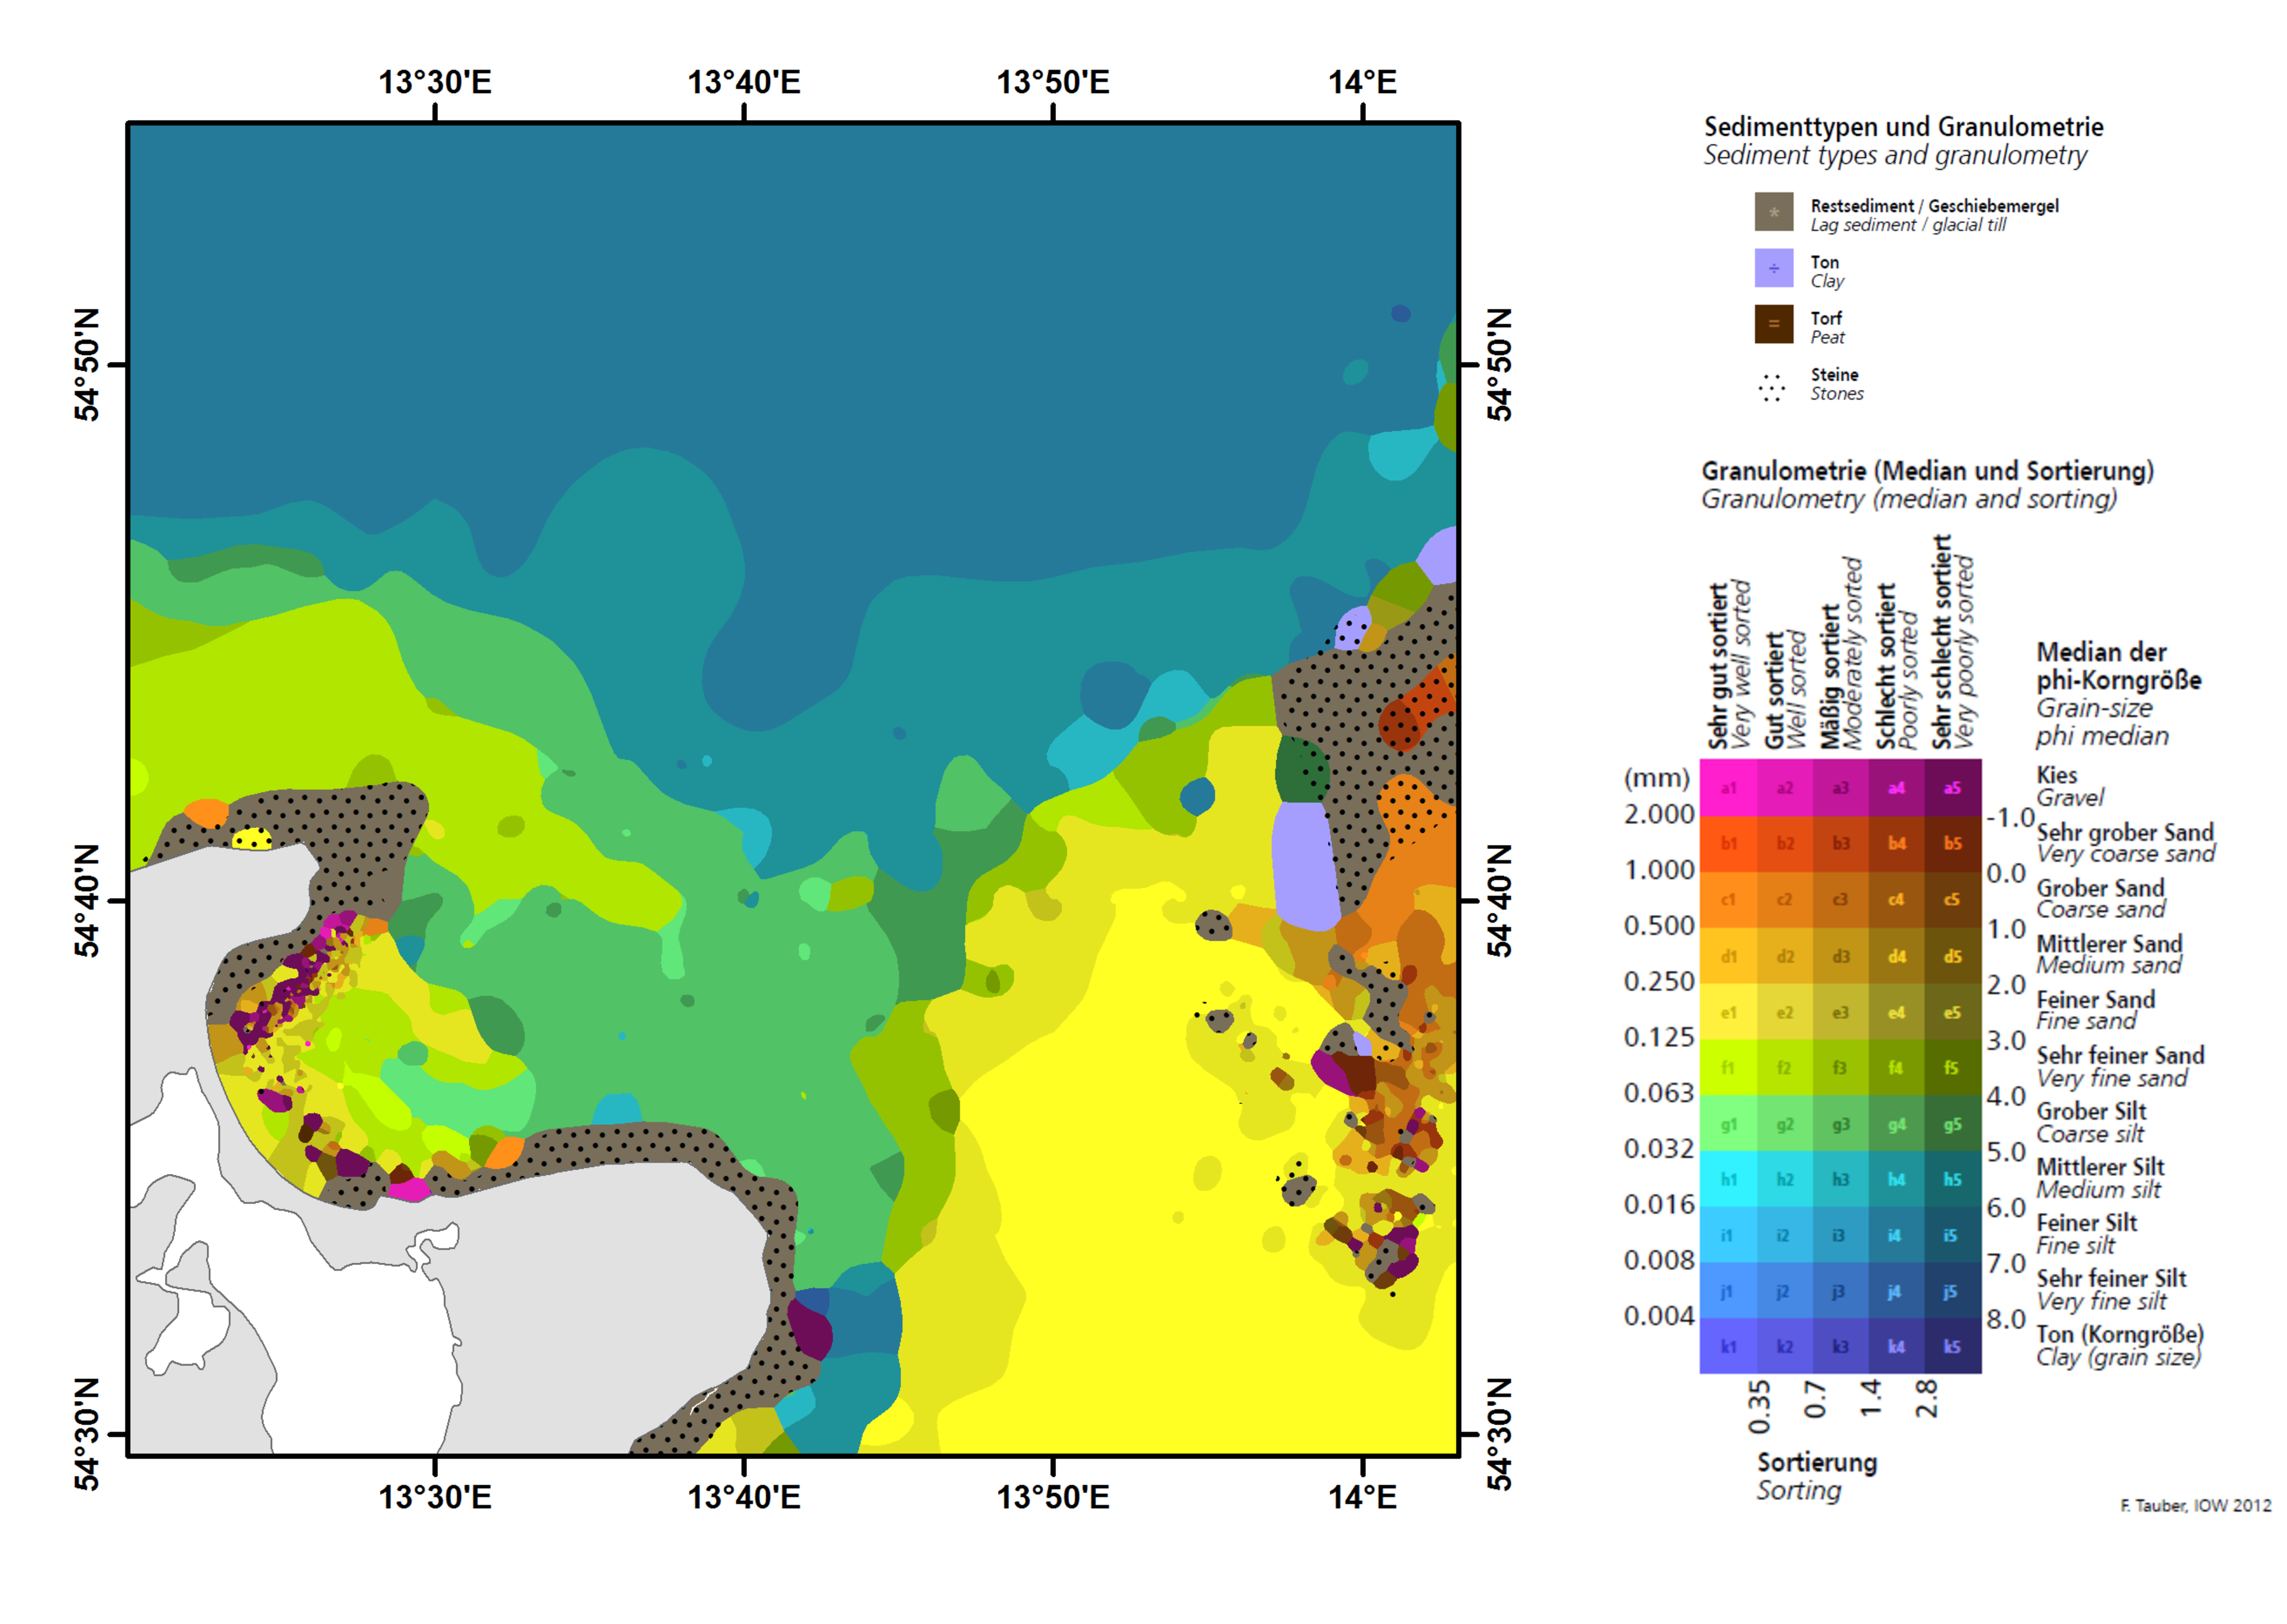
\includegraphics[width=40pc]{bilder/TW.pdf}
 \caption{Sediment distribution in the study area. Data were taken from 
\cite{tauber2012}.}
 \label{tauberkarte}
 \end{figure}

Three different types of moorings were deployed: A CTD-Chain consisted of eight 
CTD-loggers (MicroCat from Seabird, USA), tied to a mooring line at intervals 
of 1 m, starting at 1 m above the seabed, additionally two optical 
backscatter sensors (NTU from Wetlabs, USA) at 3.5 and 5.5 m above the seabed. 
For the EMB100 cruise, the CTD-Chain was extended to 10 CTD-loggers (5 MicroCat 
and 5 TR-1060 type from RBR, Canada) and the turbidity sensors were omitted. 
Lander 1 was a bottom-mounted instrument frame with an upward looking 1200 kHz 
ADCP (Teledyne RDI, USA), a 6 MHz single-point Doppler current meter (Vector 
from Nortek AS, Norway), another CTD-logger and a turbidity sensor. Lander 2 
was a similar bottom frame equipped with an upward looking 600 MHz ADCP 
(Teledyne RDI, USA) and an upward looking 1 MHz (2 MHz during cruise AL434) 
pulse-coherent ADCP (Aquadopp HR from Nortek AS, Norway). For the cruises 
EMB100 and MSM50, Lander 2 was complemented with an additional CTD-logger and a 
turbidity sensor. Deployment times of the moorings are listed in 
\tab{deployments}.

 \begin{table}
\caption{Deployment times of moorings (UTC). In the first 
line, TW and AB indicate deployment sites near the coast and in the Arkona 
Basin, respectively.}\label{deployments}
\begin{center}
\begin{tabular}{cccc}
 & AL434 (TW) & EMB100 (AB) & MSM50 (TW) \\
 \hline
 start & 03.04.2014, 07:00 & 14.04.2015, 12:00 & 26.01.2016, 22:00 \\ 
 end & 08.04.2014, 06:00 & 17.04.2015 04:00 & 28.01.2016, 07:00 \\
\hline
 & CTD-Chain & CTD-Chain & \\
 & Lander 1 & Lander 1 & Lander 1\\
 & Lander 2 & Lander 2 & Lander 2\\
\end{tabular}
\end{center}
\end{table}

Ship-based microstructure measurements were performed with a MSS90-L 
microstructure profiler (ISW, Germany). The instrument contained a set of 
precision CTD sensors, a fast FP07 thermistor, a turbidity sensor, and two 
airfoil shear-probes. During the transects (each of 1 to 5 hours duration) the 
ship moved at 1-2 kn and profiles were obtained continously. Number and time of 
the transects for each cruise are summarized in \tab{mss}.

 \begin{table}
\caption{Start and end times (UTC) and number (in brackets) of microstructure 
transects.}\label{mss}
\begin{center}
\begin{tabular}{cccc}
 & AL434 (2014) & EMB100 (2015) & MSM50 (2016)\\
 \hline
Tromper & 04.04., 16:15 - & & 27.01., 00:00 - \\ 
Wiek & 04.04., 22:30 (4) & & 28.01., 06:00 (9)\\
 & 06.04., 17:30 & & \\
 &  07.04., 22:15 (8) & & \\
\hline
Arkona & 05.04., 16:15 - & 14.04., 16:45 - & 23.01., 13:30 - \\
Basin & 06.04., 01:15 (5) & 15.04., 05:30 (5) & 24.01., 16:45 (7)\\
\hline
transect &  & & 24.01., 19:30 - 23:45 (T1)\\
coast to basin & & & 28.01., 09:45 - 17:00 (T2)\\
\end{tabular}
\end{center}
\end{table}

\section{Observations}

 \begin{figure}[ht]
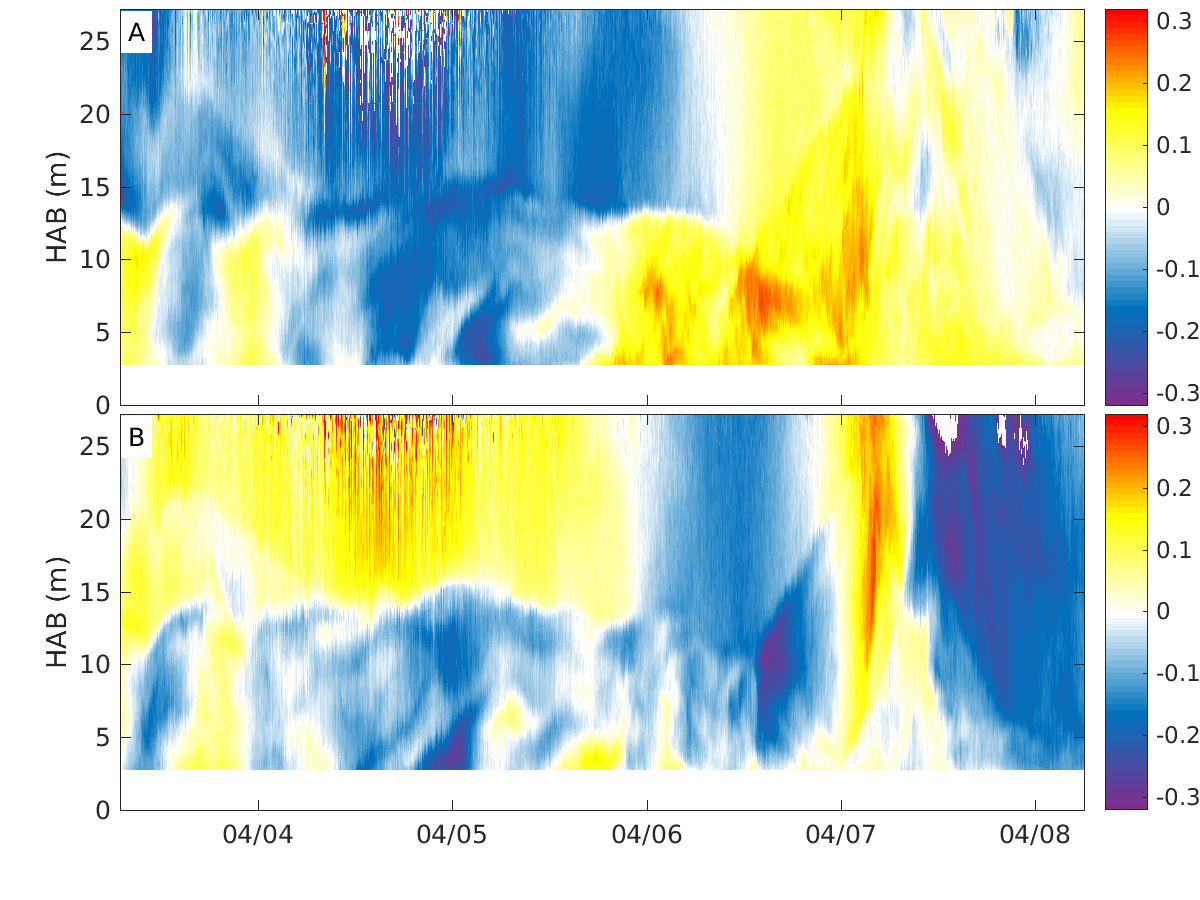
\includegraphics[width=40pc]{bilder/adcp600.png}
 \caption{Time series of velocity profiles obtained with the 600~kHz ADCP on 
Lander 2 during the deployment at TW on cruise AL434 (April 2014).}
 \label{adcp600}
 \end{figure}

\subsection{Tromper Wiek}

During the 5 day instrument deployment in 2014 (\tab{deployments}), we captured 
a storm event with 7 Bft wind and up to 4 m wave height with a consecutive calm 
period (\fig{tromperwiek}, a). In \fig{tromperwiek}, b the variance of the 
horizontal velocity componentsfiltered for wave periods between 2 and 20 
seconds, which is proportional to the kinetic energy contained in the 
waves, is displayed. Although wave energy was maximal in the afternoon of April 
4, the peak in turbidity was not reached until late morning of April, 5. This 
yields that local resuspension during storm did not occur, but a turbid 
watermass was advected to the measurement site. Near bottom current 
(\fig{tromperwiek},C) was directed to the south during the relevant period, i.e. 
water from deeper parts was advected up the slope.
 \begin{figure}[ht]
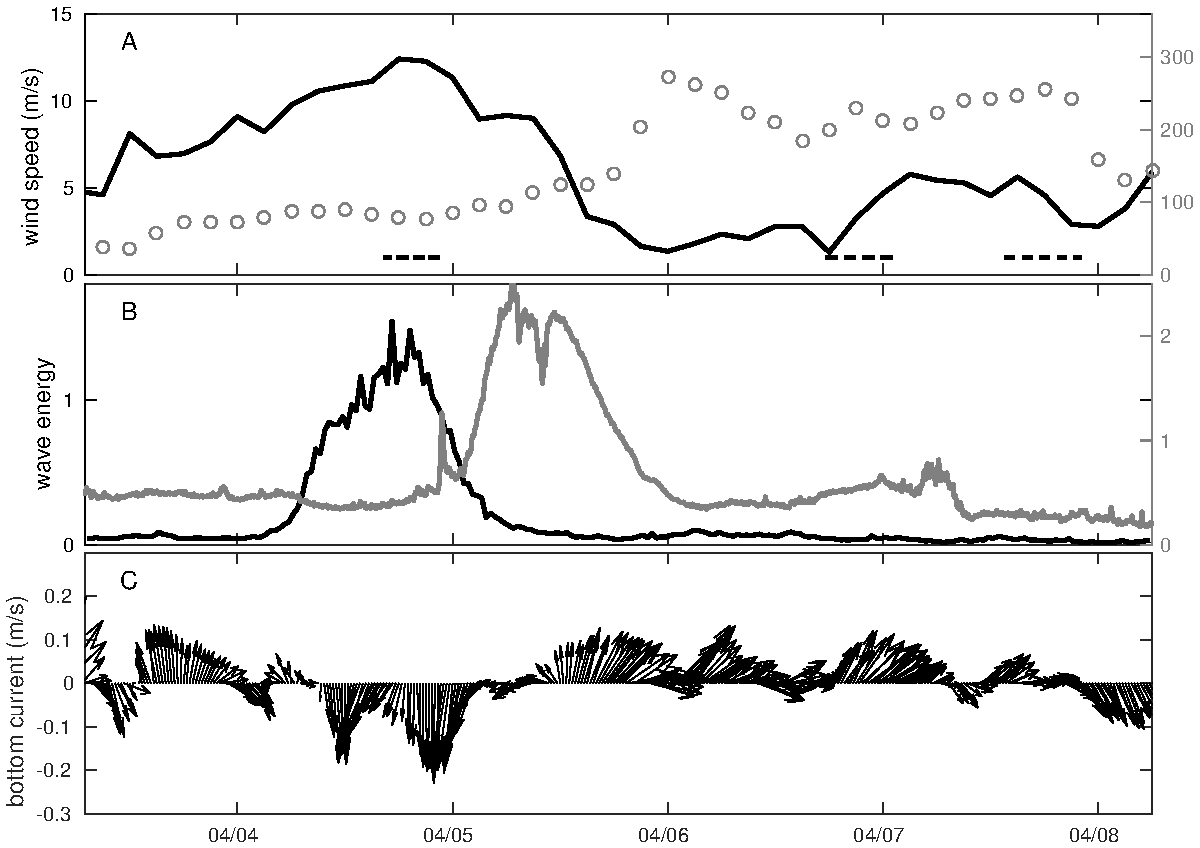
\includegraphics[width=15cm]{bilder/al434tw.pdf}
 \caption{(A) Wind speed and direction from the hindcast of the German Weather 
Service, (B) wave energy and turbidity and (C) direction of 
near bottom current, all obtained with Lander 1 during the deployment at TW on 
cruise AL434 (April 2014).}
 \label{tromperwiek}
 \end{figure}

In the CTD Chain data in \fig{ctdchain} we see a steady increase of the 
near-bottom salinity, accompanied by increasing turbidity. The increase in 
turbidity is clearly linked to the increase of salinity, supporting that turbid 
water is advected to TW from deeper regions below the halocline.

 \begin{figure}[ht]
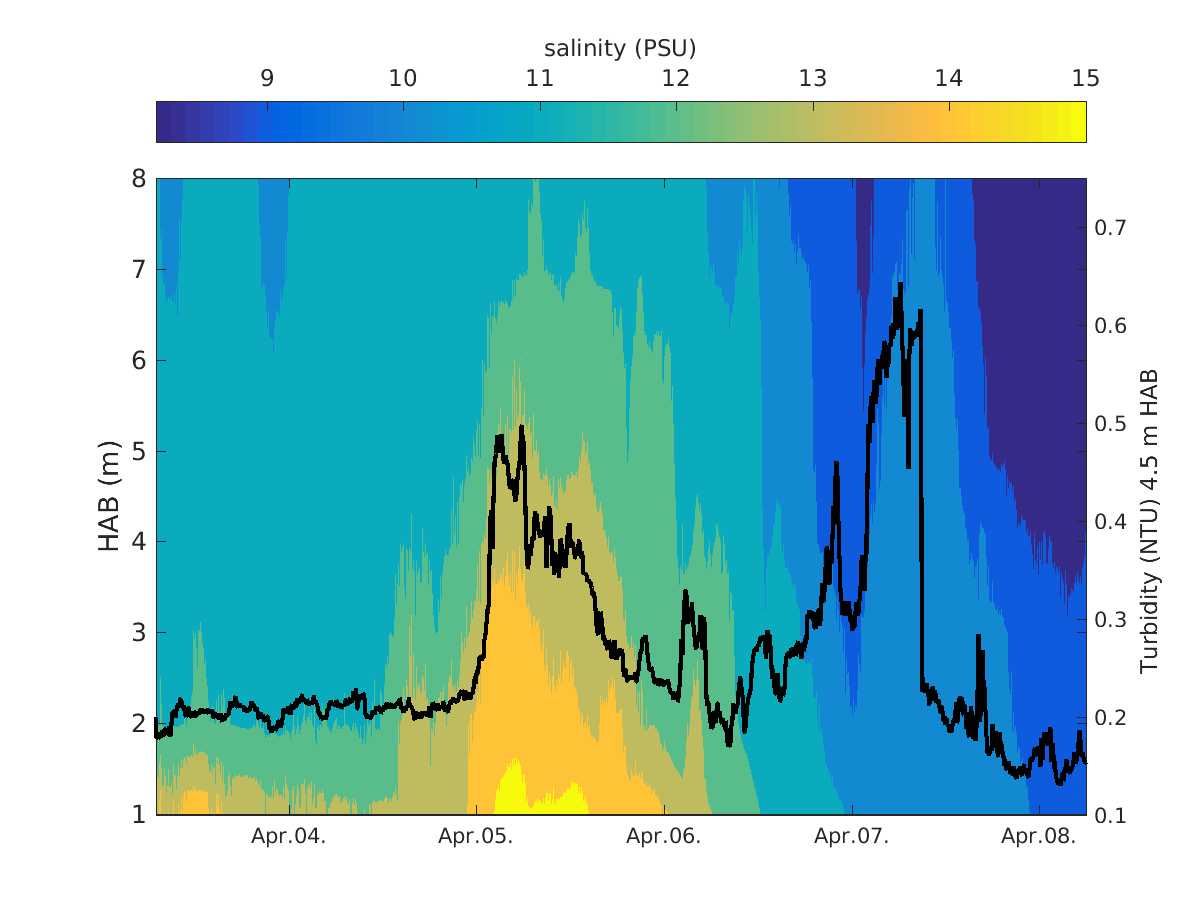
\includegraphics[width=15cm]{bilder/ctdchaintw.png}
 \caption{Salinity (PSU) obtained from the CTD Chain deployed at Tromper Wiek 
during cruise AL434.}
 \label{ctdchain}
 \end{figure}

 This advection of saline water near the bottom is triggered by the local wind 
forcing. Strong easterly wind causes Ekman transport to the north in the 
surface layer \citep[][]{lass2001}, which is visible in the velocity data from 
the 600~kHz ADCP mounted on Lander~2. After the wind decayed, 

\subsection{Transect}

In \fig{transect} we see how the water body is structured along the slope from 
the coast into the basin. A sharp halocline seperates a turbulent bottom 
boundary layer (BBL) of approximately 5 m from the interior. At the left hand 
side of the pannel, where the slope angle steepens, the halocline is widened. 
The boundary layer is generally turbid: Turbidity is more patchy at the upper 
parts of the slope, but high values are confined to the bottom boundary layer, 
so no suspended matter is mixed across the halocline. This indicates that 
turbidity is caused by material originating from the seafloor and held in 
suspension by turbulent motions in the BBL.
Salinity isolines are rather parallel to the slope than straight horizontal, 
what would be the stably stratified case.
  \begin{figure}[ht]
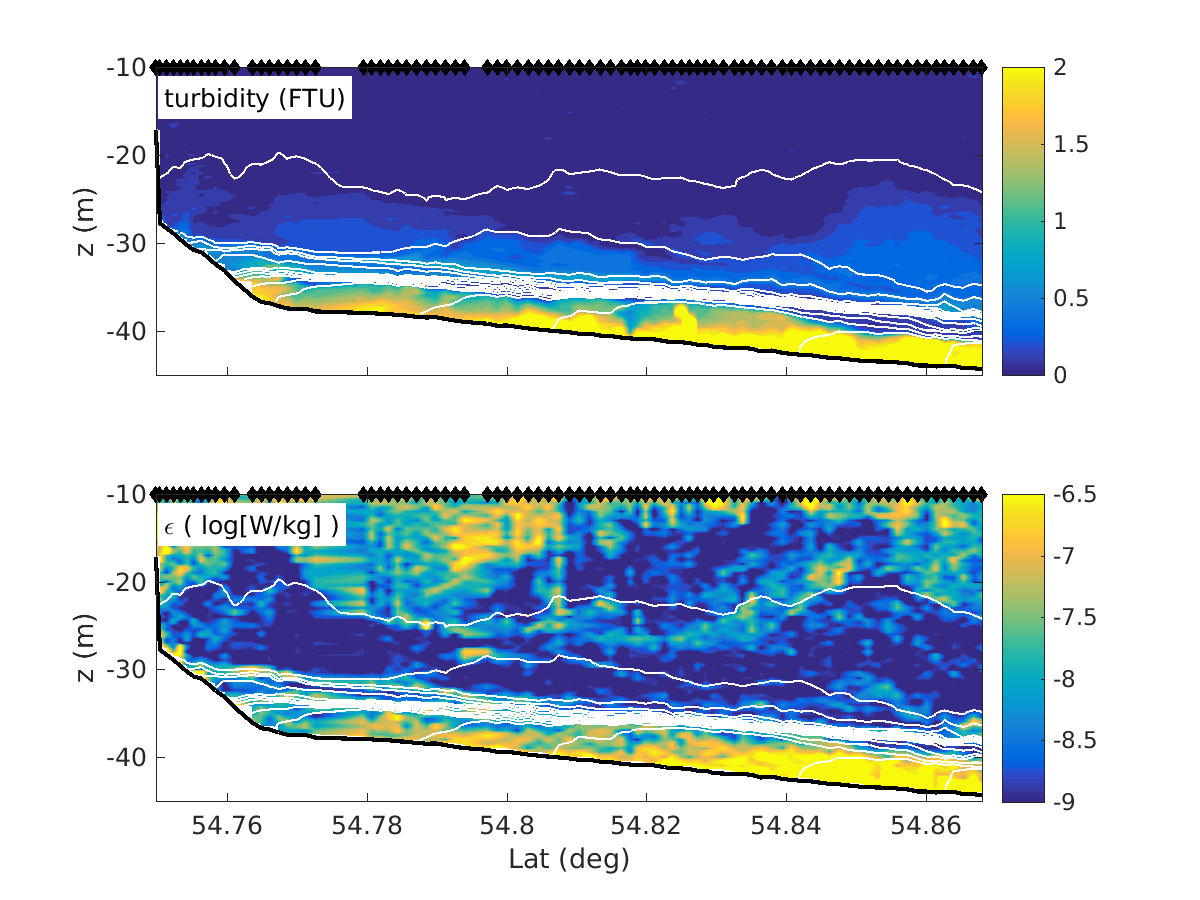
\includegraphics[width=40pc]{bilder/abtrans.png}
 \caption{Turbidity and dissipation rate from the microstructure transect T1. 
White lines indicate levels of equal salinity.}
 \label{transect}
 \end{figure}


\subsection{Arkona Basin}

During each of the three cruises, we collected microstructure data in the 
Arkona Basin. \fig{abmss} shows the profiles of dissipation rate and turbidity, 
averaged over all profiles obtained in the basin for each cruise. A turbulent 
BBL is visible in all three profiles, ranging from 1 to 5 m thickness. 
Turbidity is again enhanced in the BBL, but not above, supporting the data 
described in the last section. As this data set was obtained over three years 
and in different seasons, it is most likely that this turbid, very sharply 
defined BBL is constantly present in the Arkona Basin.
   \begin{figure}[ht]
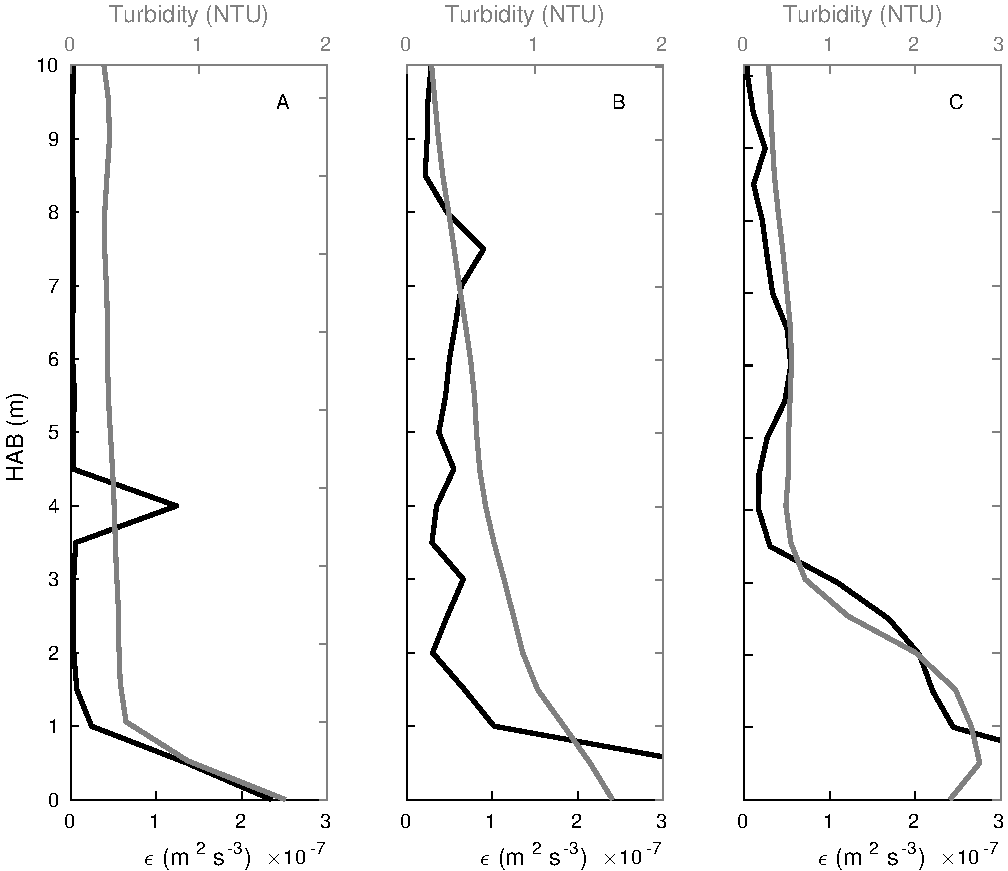
\includegraphics[width=15cm]{bilder/arkona_mss.pdf}
 \caption{Turbidity and dissipation rate from all microstructure transect in 
the Arkona Basin. Solid lines are mean values, dashed line the standard 
deviation. Only the lowermost part of the watercolumn is displayed here.}
 \label{abmss}
 \end{figure}
 
\section{Discussion}

\section{Conclusions}
\end{mainmatter}

% Anhaenge -- auskommentieren falls nicht ben\"{o}tigt.
\begin{appendices}
\chapter{Numerical boundary conditions for SPM concentrations}
\pagenumbering{roman}

In view of the strong near-bottom gradients of suspended material, the
implementation of the boundary conditions for the SPM transport
equation \eq{c} requires special attention. While \eq{defFz} provides
an exact expression for the upward turbulent flux $F_z$ at the bottom,
the numerical implementation of the sinking flux,
\begin{equation}
 \label{Fs}
 F_s(z=0) = w_s c_0 \comma
\end{equation}
is not straightforward because the bottom concentration, $c_0$, is
unknown. In vertically staggered numerical grids typically used in
ocean modeling, the bottom concentration $c_0$ has to be estimated
from the known concentration $c_1$ in the center of the lowermost grid
cell, which requires some assumptions about the vertical distribution
of the suspended material in the near-bottom region. While it is
reasonable to assume that the bottom cell is well mixed (i.e.,
$c_0=c_1$) if the bed stress $|\tau_b|$ is smaller than the critical
stress for erosion, $\tau_c$, it is likely that the bottom
concentration $c_0$ is significantly larger than $c_1$ if active
erosion takes place ($|\tau_b| > \tau_c$). In this case, the popular
assumption $c_0=c_1$ may lead to large numerical errors, and to a grid
dependence of the numerical solution. In the following, we show how a
more consistent lower boundary condition can be derived.

We start from the observation that close to the bottom, the transport
equation in \eq{c} reduces to a balance between upward mixing and
downward sinking of suspended material,
\begin{equation}
 \label{cstationary}
 0 = \nu_t^b \partder{c}{z} + w_s c
 \comma
\end{equation}
assuming small slopes ($\alpha \ll 1$) for simplicity. The turbulent
viscosity in the near-bottom region is known to follow the
law-of-the-wall relation $\nu_t = \kappa u_\ast (z + z_0)$, where
$\kappa \approx 0.4$ is the von K{\'a}rm{\'a}n constant, and $u_\ast =
|\tau_b|^{1/2}$ the bottom friction velocity
\citep[e.g.,][]{Pope2000a}. The turbulent diffusivity $\nu_t^b$ in this
region is proportional to $\nu_t$, and therefore adopts the form
$\nu_t^b = Pr_t^{-1} \kappa u_\ast (z + z_0)$, where the turbulent
Prandtl number, $Pr_t$, plays the role of a constant proportionality
factor of order 1. The turbulence model used in our study has been shown to
exactly reproduce this near-wall behavior for $\nu_t$ and $\nu_t^b$
\citep[e.g., ][]{UmlaufBurchard2003a,UmlaufBurchard2005a}.

Inserting the above law-of-the-wall relation for $\nu_t^b$ into
\eq{cstationary}, we find a solution of the form
\begin{equation}
 \label{Rouse}
 \dfrac{c}{c_0} = \left( \frac{z}{z_0} + 1 \right)^{-p} \comma
\end{equation}
which is recognized as the classical Rouse profile
\citep{vanRijn84b}, slightly modified here by the appearance of the
turbulent Prandtl number in the definition of the Rouse number $p =
w_sPr_t \, / (\kappa u_\ast)$.

Recalling that in any conservative numerical scheme, $c_1$ represents
the average concentration inside the lowermost grid cell, a relation
between $c_0$ and $c_1$ may be found from integrating \eq{Rouse}
across the cell. If we denote $h$ as the cell thickness, this yields
\begin{equation}
 \label{cbot}
 c_0 = \frac{c_1}{r} \quad \text{for} \quad |\tau_b|>\tau_c \comma
\end{equation}
where 
\begin{equation}
 \label{rr}
 r =  \frac{1}{(1-p) h/z_0} \left[ \left( \frac{h}{z_0} + 1 \right)^{1-p} -1 \right] 
 \comma
\end{equation}
\begin{figure}[ht]
  \noindent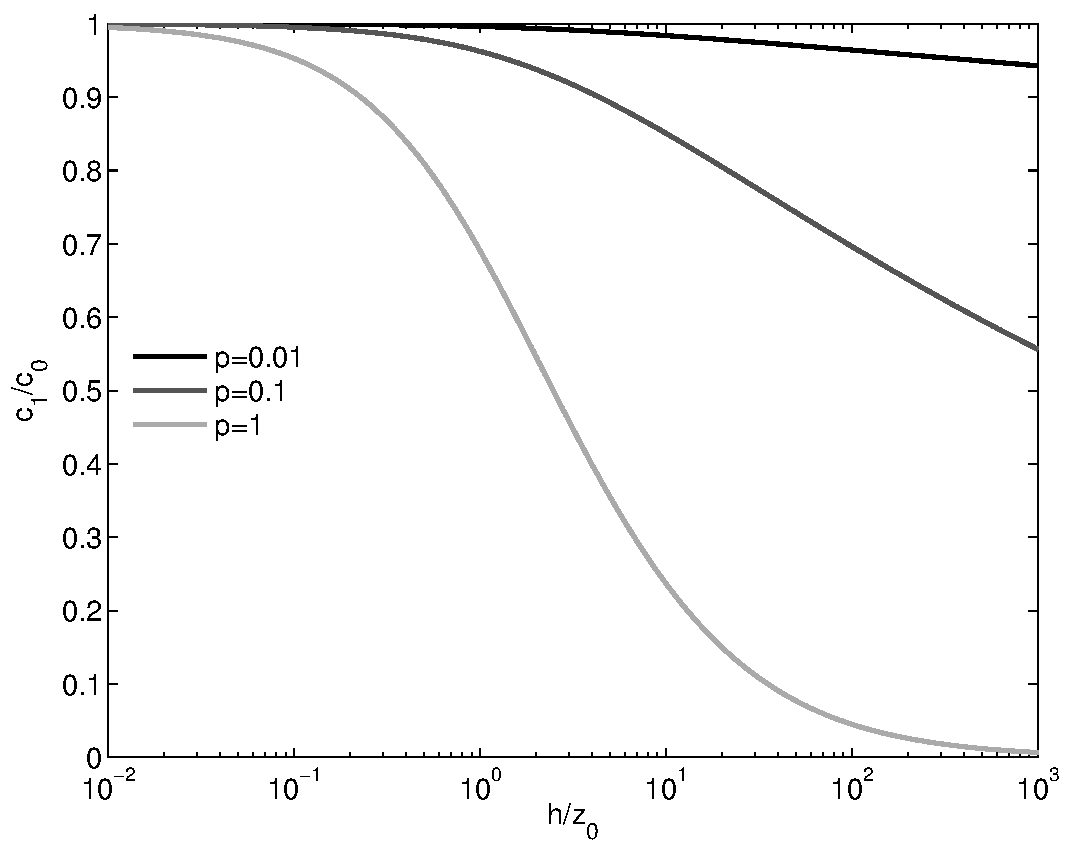
\includegraphics[width=29pc,angle=0]{bilder/rouse.pdf}\\
  \caption{A1}{Concentration ratio $c_1/c_0$ as a function of
    non-dimensional cell thickness, $h/z_0$, for different Rouse
    numbers according to \eq{cbot}.\label{c0c1}}
\end{figure}
Fig. A1 shows the ratio $r=c_1/c_0$ as a function of the normalized
cell thickness $h/z_0$ for different Rouse numbers. The most important
conclusion from this figure is that the naive approach of assuming
$c_0 = c_1$ to compute the sinking flux in \eq{Fs} during erosion
periods introduces large numerical errors except for small Rouse
numbers and/or extremely fine grids with $h \ll z_0$. Below, we
nevertheless discuss some reference solutions that satisfy this
condition. We note, however, that the constraint $h \ll z_0$ implies
$\Delta t \ll z_0 / w_s$ for the numerical time step according to the
well-known CFL stability criterion for explicit advection schemes. It
is easy to show that, even for idealized one-dimensional simulations,
the numerical effort may become prohibitively large for small $z_0$.

Using the example from Section \ref{sec:bbl} above, Fig. A2
illustrates that assuming $c_0 = c_1$ during both erosive and
non-erosive periods leads to significant numerical errors, and to a
grid-dependence of the results. 
\begin{figure}[ht]
  \noindent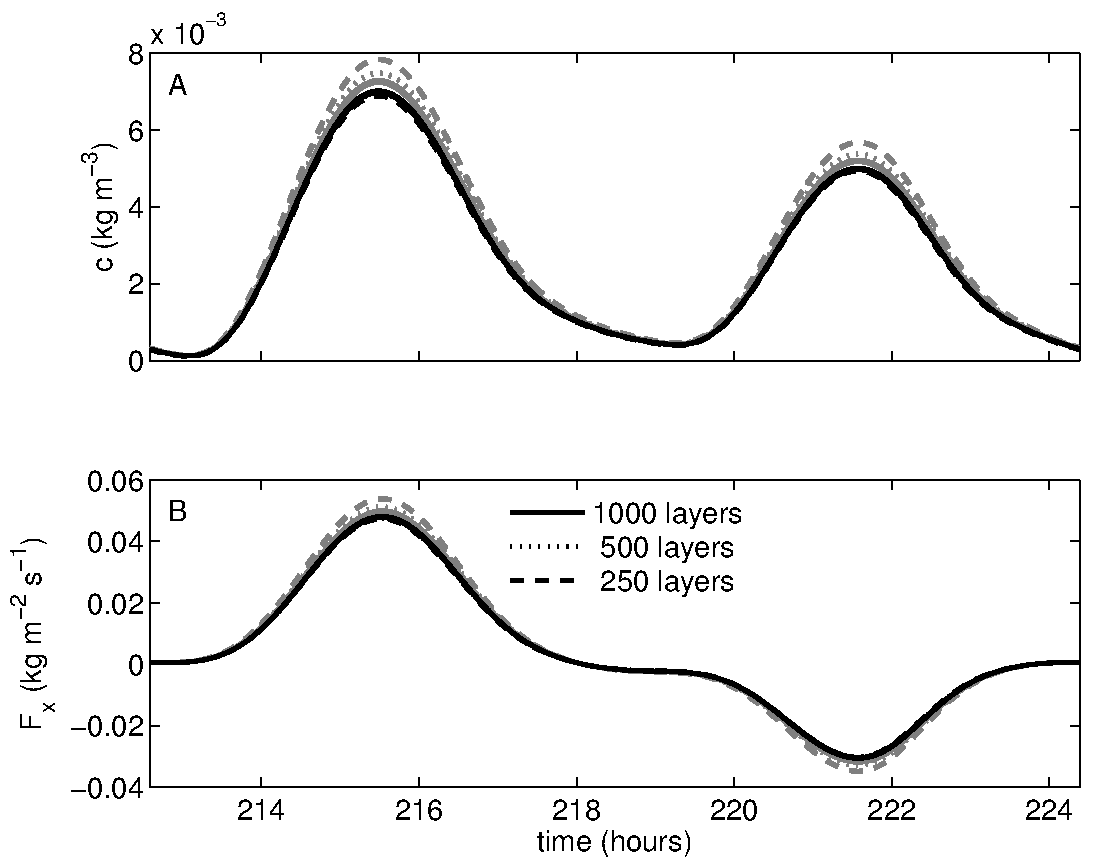
\includegraphics[width=29pc,angle=0]{bilder/appendix.pdf}\\ \caption{A2}{Numerical
    results for (a) SPM concentration 5~m above the bottom, and (b)
    upslope flux $F_x$ for three vertical resolutions. Gray lines are
    based on the assumption $c_0 = c_1$ to compute the sinking flux in
    \eq{Fs}, whereas black lines are based on \eq{cbot} during erosive
    periods. Parameters correspond to Case 1 in
    \tab{params}. \label{convergence}}
\end{figure}
Estimating $c_0$ based on \eq{cbot}
during periods with active erosion, however, removes this dependency
on the numerical grid, and leads to stable results already for
moderate vertical resolution. All results discussed in this manuscript
are therefore based on this new expression. Convergence studies were
carried out to insure that all our results are independent of the
numerical grid size and time step.
\end{appendices}

\begin{backmatter}
% Verweis auf Literaturverzeichnis zum Inhaltsverzeichnis hinzufuegen
\addtocontents{toc}{\vspace*{1em}}

% Literaturliste aus Literaturdatenbank (Bibtex-Datei) bauen. Nur tatsaechlich zitierte Literatur wird in Liste aufgenommen.
% Regelmaessigen Aufruf von ``bibtex abschlussarbeit'' nicht vergessen, falls das der Latex-Editor nicht
% erledigt.
% Zur Bearbeitung der Literaturdatenbank kann das Programm JabRef (http://jabref.sf.net) empfohlen werden. (Java-Programm, laeuft unter Windows, Linux, Mac, ...)
\bibliography{literatur}
% Stil fuer Literaturliste festlegen
% Variante A: DIN, Eintraege erhalten Kuerzel aus Autoren-Initialien und Jahr, alphabetisch geordnet
% \bibliographystyle{alphadin}
% Variante B: DIN, Eintraege werden durchnummeriert, alphabetisch geordnet
\bibliographystyle{ametsoc2014}


\begin{abstract}[Selbständigkeitserklärung]
\thispagestyle{empty}
Ich versichere hiermit an Eides statt, dass ich die vorliegende Arbeit selbstständig
angefertigt und ohne fremde Hilfe verfasst habe, keine außer den von mir
angegebenen Hilfsmitteln und Quellen dazu verwendet habe und die den benutzten
Werken inhaltlich und wörtlich entnommenen Stellen als solche kenntlich gemacht
habe.
\vspace*{2cm}

\flushright{
Rostock, (\today)
}
\end{abstract}

\end{backmatter}

\end{document}
